\section{Introduction}
Large language models (LLMs) have shown great performance in many NLP tasks \citep{brown2020language,bang2023multitask}. What's especially striking is their ability to handle complex tasks through reasoning \citep{wei2022chain,huang2022towards}. To further unleash LLMs' reasoning ability, the plan-and-solve paradigm \citep{wang2023plan} has been proposed, in which LLMs are prompted to generate a plan and execute each reasoning step. In this way, LLMs decompose complex reasoning tasks into a series of sub-tasks and solve them step by step \citep{khot2022decomposed}. 

Despite their success, LLMs are still limited by the lack of knowledge and prone to hallucinations during reasoning, which can lead to errors in reasoning processes \citep{hong2023faithful,wang2023knowledge}. For example, as shown in \Cref{fig:intro}, LLMs do not have the latest knowledge and hallucinate an incorrect reasoning step: ``has a daughter''. These issues largely diminish the performance and trustworthiness of LLMs in high-stakes scenarios, such as legal judgment and medical diagnosis. 

To tackle the issues, knowledge graphs (KGs) have been incorporated to improve the reasoning ability of LLMs \citep{pan2023unifying,luo2023chatrule}. KGs capture abundant factual knowledge in a structured format, which provides a faithful knowledge source for reasoning. As a typical reasoning task, knowledge graph question answering (KGQA) aims to obtain answers based on knowledge from KGs \citep{sun2019pullnet}. Previous works that jointly use KGs and LLMs for KGQA reasoning can be broadly divided into two categories: 1) semantic parsing methods \citep{lan2020query,ye2022rng}, which use LLMs to convert questions into logical queries that are executed on KGs to obtain answers; and 2) retrieval-augmented methods \citep{li2023graph,jiang2023reasoninglm}, which retrieve triples from KGs as knowledge context and uses LLMs to obtain the final answers. 

Although semantic parsing methods can generate more accurate and interpretable results by leveraging reasoning on KGs, the generated logical queries can often be non-executable and yield no answers, due to syntax and semantic limitations \citep{yu2022decaf}. Retrieval-augmented methods are more flexible and exploit the ability of LLMs for reasoning. However, they only treat KGs as factual knowledge bases and overlook the importance of their structural information for reasoning \citep{jiang2022unikgqa}. For instance, as shown in \Cref{fig:intro}, a \emph{relation path}, which is a sequence of relations, ``\texttt{child\_of}$\to$\texttt{has\_son}'' can be used to obtain answers to the question ``Who is the brother of Justin Bieber?''.  Therefore, it is essential to enable LLMs to directly reason on KGs to achieve faithful and interpretable reasoning.

In this paper, we propose a novel method called reasoning on graphs (\ourmethod) that synergizes LLMs with KGs to conduct faithful and interpretable reasoning. To \RE{alleviate} the issues of hallucinations and lack of knowledge, we present a \emph{planning-retrieval-reasoning} framework, where \ourmethod first generates relation paths grounded by KGs as faithful plans via the \emph{planning module}. These plans are then used to retrieve valid reasoning paths from KGs to conduct faithful reasoning by the \emph{retrieval-reasoning module}. In this way, we not only retrieve the latest knowledge from KGs but also consider the guidance of KG structure for reasoning and explanations. Moreover, the planning module of \ourmethod can be plug-and-play with different LLMs during inference to improve their performance.
%
Based on this framework, \ourmethod is optimized by two tasks: 1) \emph{planning optimization}, where we distill knowledge from KGs into LLMs to generate faithful relation paths as plans; and 2) \emph{retrieval-reasoning optimization}, where we enable LLMs to conduct faithful reasoning based on retrieved paths and generate interpretable results. We conduct extensive experiments on two benchmark KGQA datasets, and the results demonstrate that \ourmethod achieves state-of-the-art performance on KG reasoning tasks and generates faithful and interpretable reasoning results.
\begin{figure}[]
    \begin{center}
    %\framebox[4.0in]{$\;$}
    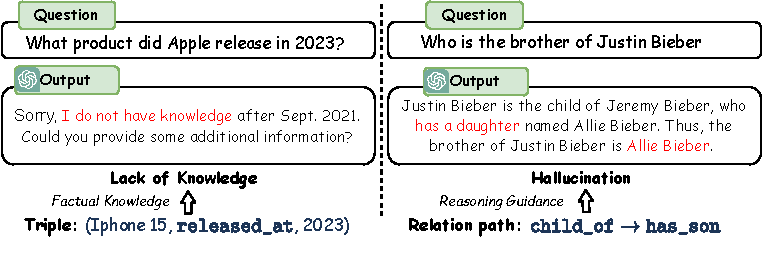
\includegraphics[width=.8\columnwidth,trim=0 0.3cm 0 0,clip]{images/intro.pdf}
    \end{center}
    \vspace{-4mm}
    \caption{The issues of lack of knowledge and hallucination in LLMs reasoning and how they can be addressed by triples and relation paths from KGs.}
    \label{fig:intro}
    \vspace{-5mm}
\end{figure}